\documentclass[11pt]{article}

\usepackage{geometry}
\usepackage{subcaption} 
\geometry{letterpaper}

\usepackage{doc}
\usepackage{cite}
\usepackage[margin=1cm]{caption}

\usepackage{url}

\usepackage{graphicx}

\title{Dream Design}
\author{Trixie Roque}
\date{11/24/2015}

\begin{document}
\maketitle

\begin{abstract}
The purpose of this paper is to design a new user interface for the Instagram application by integrating timeline options similar to the ones employed by Facebook, as well as allowing the users more freedom in their posts.
\end{abstract}

\pagebreak
\tableofcontents

\pagebreak

\section{Introduction}
\label{Introduction}
    \indent Social media applications have become a common tool in our society, especially to millennials. The ability to connect with both friends and strangers alike through the submission of "posts" onto the internet has become so widespread that it is rare to find a person that do not possess at least one social media account. Some people can even say that their hobbies involve sifting through countless blogs, tweets, videos, etc. of internet celebrities. Because of the easy access that social media applications provide us to peek through the various adventures in other people's lives, we have become incredibly immersed in them. However, even with the continuous appearance of various applications that aim to grab our everyday attention, design flaws can still exist. \\
     \indent Today's social media posts often involve clever quips, funny memes, or embarrassingly hilarious gifs or videos. 
\\
    \indent Therefore, in order to address the issues with respect to the interface design of Instagram.


\section{System Description}
\label{System Description}
Although there is a desktop client for Instagram, the main focus of this paper is to address the designs in the mobile application. 

\section{Top-Level Design}
The design would incorporate the Google Maps API and the Instagram API into a conglomeration that allows for posts, as well as 
The application will employ Snapchat's feature that allows the user to draw on the images. Currently, Instagram only allows various filters other lighting adjustments

\begin{figure}[ht]
\centering
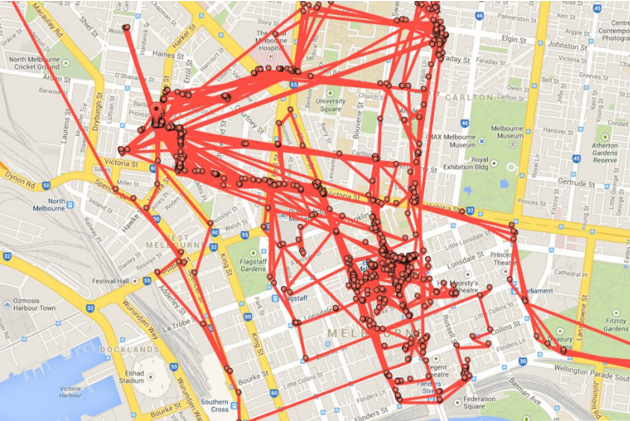
\includegraphics[width=5in]{images/google_maps_tracking.png}
\label{google_tracking}
\end{figure}

\begin{figure}[ht]
\centering
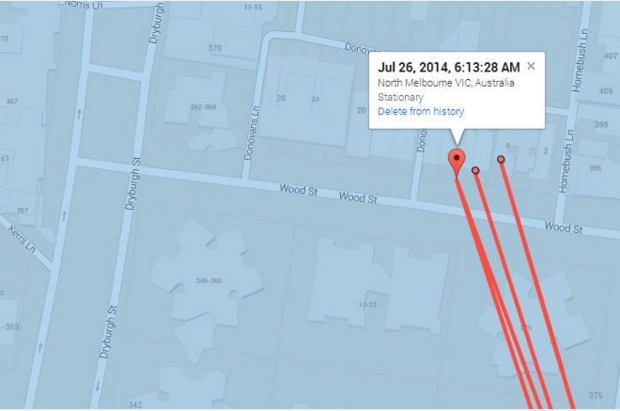
\includegraphics[width=5in]{images/google_maps_tracking_with_info.png}
\label{google_tracking}
\end{figure}

\begin{figure}[ht]
\centering
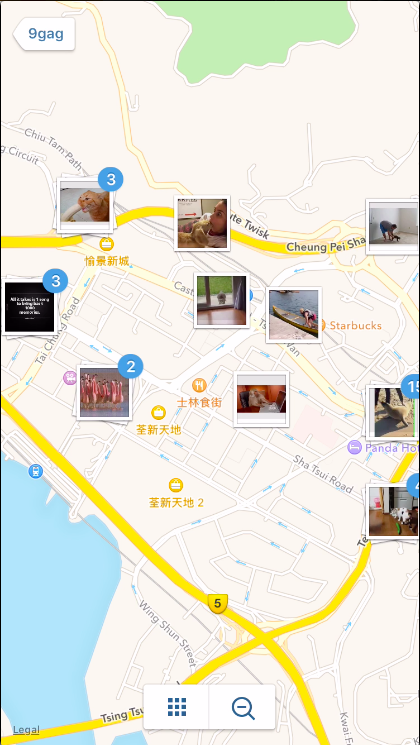
\includegraphics[height=5in]{images/maps_with_pictures.png}
\label{google_tracking}
\end{figure}

\begin{figure}[ht]
\centering
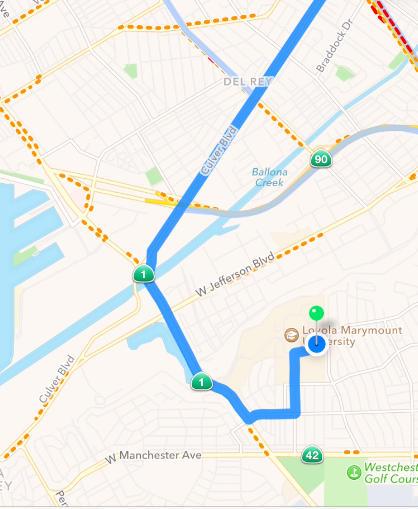
\includegraphics[width=3in]{images/gps.png}
\label{google_tracking}
\end{figure}

\begin{figure}[ht]
\centering
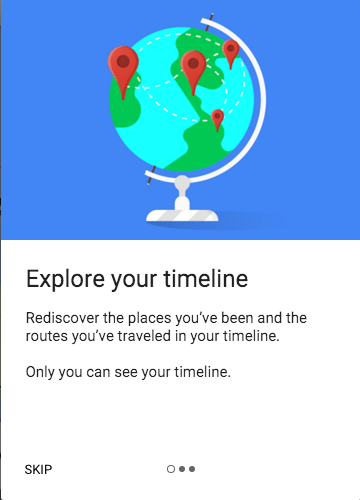
\includegraphics[width=3in]{images/view_your_timeline_prompt.png}
\label{google_tracking}
\end{figure}

\section{Usage Scenarios}

\section{Rationale}

\section{Usability Metric ``Forecast''}
Since the new design would integrate features that other APIs present, the usability metrics would have to be discussed. If the designs are successfully implemented and tested, given enough time, money, and manpower, the strongest metrics would have to be 
\indent Because of the added features, the number of errors would definitely increase since the user would have more options to tap a button they did not intend to select. 
\indent However, the strongest suit of the interface, in terms of the usability metrics discussed in class, would be satisfaction and efficiency. Because the purpose of the interface is to allow the users more freedom for their posts, consumer satisfaction is a necessary metric to fulfill. Additionally, since the interface would be implemented into a social media application, if it becomes widely used, then an expert user can easily navigate through the application's optional features.

\clearpage

\bibliographystyle{plain}
\end{document}

\end{document}